%%%%%%%%%%%%%%%%%%%%%%%%%%%%%%%%%%%%%%%%%
% baposter Landscape Poster
% LaTeX Template
% Version 1.0 (11/06/13)
%
% baposter Class Created by:
% Brian Amberg (baposter@brian-amberg.de)
%
% This template has been downloaded from:
% http://www.LaTeXTemplates.com
%
% License:
% CC BY-NC-SA 3.0 (http://creativecommons.org/licenses/by-nc-sa/3.0/)
%
%%%%%%%%%%%%%%%%%%%%%%%%%%%%%%%%%%%%%%%%%

%----------------------------------------------------------------------------------------
%	PACKAGES AND OTHER DOCUMENT CONFIGURATIONS
%----------------------------------------------------------------------------------------

\documentclass[landscape,a0paper,fontscale=0.3]{baposter} % Adjust the font scale/size here

\usepackage{xcolor}
\usepackage{natbib} % for bibliography
\usepackage{graphicx} % Required for including images
\graphicspath{{figures/}} % Directory in which figures are stored

\usepackage{amsmath} % For typesetting math
\usepackage{amssymb} % Adds new symbols to be used in math mode

\usepackage{booktabs} % Top and bottom rules for tables
\usepackage{enumitem} % Used to reduce itemize/enumerate spacing
\usepackage{palatino} % Use the Palatino font
\usepackage[font=small,labelfont=bf]{caption} % Required for specifying captions to tables and figures
\usepackage{outlines} % for nested lists
\usepackage{capt-of} % side-by-side figure and table
\usepackage{multicol} % Required for multiple columns
\usepackage{tikz}

%% Citation packages
\usepackage{natbib}

%%%%%%%% Custom commands
\usepackage{mycommands}

\setlength{\columnsep}{1.5em} % Slightly increase the space between columns
\setlength{\columnseprule}{0mm} % No horizontal rule between columns

\usepackage{tikz} % Required for flow chart
\usetikzlibrary{shapes,arrows} % Tikz libraries required for the flow chart in the template

\newcommand{\compresslist}{ % Define a command to reduce spacing within itemize/enumerate environments, this is used right after \begin{itemize} or \begin{enumerate}
\setlength{\itemsep}{1pt}
\setlength{\parskip}{0pt}
\setlength{\parsep}{0pt}
}

\definecolor{lightblue}{rgb}{0.145,0.6666,1} % Defines the color used for content box headers
\definecolor{umnmaroon}{RGB}{122,0,25}
\definecolor{umngold}{RGB}{255,204,51}
\newcommand{\colmarit}{\color{umnmaroon} \it}
\newcommand{\colmarbf}{\color{umnmaroon} \bf}

% Row color change in table
\makeatletter
\def\zapcolorreset{\let\reset@color\relax\ignorespaces}
\def\colorrows#1{\noalign{\aftergroup\zapcolorreset#1}\ignorespaces}
\makeatother
\begin{document}

\begin{poster}
{
headerborder=closed, % Adds a border around the header of content boxes
colspacing=1em, % Column spacing
bgColorOne=lightblue, % Background color for the gradient on the left side of the poster
bgColorTwo=white, % Background color for the gradient on the right side of the poster
borderColor=umnmaroon, % Border color
headerColorOne=umnmaroon, % Background color for the header in the content boxes (left side)
headerColorTwo=umngold, % Background color for the header in the content boxes (right side)
headerFontColor=white, % Text color for the header text in the content boxes
boxColorOne=white, % Background color of the content boxes
textborder=roundedleft, % Format of the border around content boxes, can be: none, bars, coils, triangles, rectangle, rounded, roundedsmall, roundedright or faded
eyecatcher=true, % Set to false for ignoring the left logo in the title and move the title left
headerheight=0.1\textheight, % Height of the header
headershape=roundedright, % Specify the rounded corner in the content box headers, can be: rectangle, small-rounded, roundedright, roundedleft or rounded
headerfont=\Large\bf\textsc, % Large, bold and sans serif font in the headers of content boxes
%textfont={\setlength{\parindent}{1.5em}}, % Uncomment for paragraph indentation
linewidth=2pt % Width of the border lines around content boxes
}
%----------------------------------------------------------------------------------------
%	TITLE SECTION 
%----------------------------------------------------------------------------------------
%
{
\includegraphics[height=4em]{umnlogo1}} % First university/lab logo on the left
{\huge{\bf\textsc{Identifying Driving Factors Behind Indian Monsoon Precipitation using Model Selection based on Data Depth}}
\vspace{0.1em}} % Poster title
{\large \textsc{Subhabrata Majumdar} (majum010@umn.edu), \textsc{Lindsey Dietz} (diet0146@umn.edu),
\textsc{ and Snigdhansu Chatterjee} (chatterjee@stat.umn.edu)
\\University of Minnesota Twin Cities, School of Statistics}
{
\includegraphics[height=4em]{umnlogo1}} % Second university/lab logo on the right
\vspace{.1em}

%----------------------------------------------------------------------------------------
%	INTRODUCTION
%----------------------------------------------------------------------------------------

\headerbox{Introduction}{name=objectives,column=0,row=0}{

\noindent\textbf{Objective}: Selection of important predictors behind Indian Monsoon rainfall, and using them to build a predictive model.
\vspace{.3em}

\noindent\textbf{Challenges for covariate selection}:
\begin{itemize}[leftmargin=*]\compresslist
\item Several sources of variability, e.g. variation across years and weather station;
\item Potentially heteroskedastic error structure;
\item Linearity or other regression assumptions are not guaranteed to hold and are hard to verify;
\item Huge number of possible models ($2^p$) for even moderate number of predictors ($p$).
\end{itemize}
\vspace{.3em}

\noindent\textbf{Our solution}: Use a novel model selection criterion based on data depth that works on a wide range of models, and {\colbbf selects important predictors by comparing only $p+1$ models}.
% When there are two boxes, some whitespace may need to be added if the one on the right has more content
}

%----------------------------------------------------------------------------------------
%	METHODS
%----------------------------------------------------------------------------------------

\headerbox{{\large Depth-based model selection}}{name=methods,column=1,row=0}{

\begin{center}
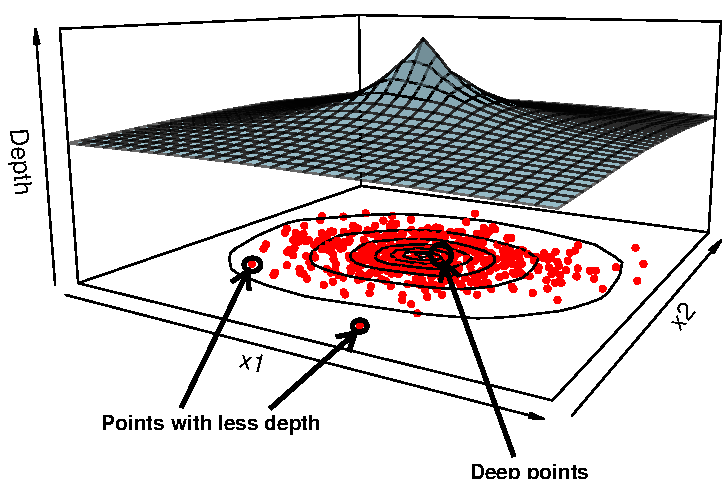
\includegraphics[width=0.8\linewidth]{depthplot_cropped}
\vspace{-2em}
\captionof{figure}{{\scriptsize Samples from bivariate normal and their depths: points away from center have less depth while those close to center have more depth}}
\end{center}

{\large {\colbbf Data depth}}

A nonparametric, scalar measure of centrality for a point $\bfx$ in sample space with respect to a data cloud $\bfX$ or probability  distribution $F$: denoted by $D(\bfx, \bfX)$ or $D(\bfx, F)$, respectively \citep{ZuoSerfling00c}.

\vspace{1em}
{\large {\colbbf The selection criterion}}

In any regression setup, consider estimators of the coefficient $\bfbeta$ based on a sample of size $n$ having elliptical sampling distributions $F_n$ centered at $\bfbeta$ that approach unit mass at $\bfbeta$ as $n \rightarrow \infty$.

\vspace{.3em}
For a candidate model, uniquely specified by its non-zero index set $\alpha$, define
\vspace{-.5em}
$$ C_n (\alpha) = \mathbb E \left[ D \left( \tilde \bfbeta_\alpha, F_n \right) \right] $$
where $\tilde \bfbeta_\alpha$ is estimate of truncated coefficient vector $\bfbeta_\alpha$, concatenated with 0 at indices not in $\alpha$.

\vspace{.3em}
Suppose $\alpha_0$ is the smallest correct model. Then:

\vspace{-.5em}
\begin{itemize}[leftmargin=*]\compresslist
\item For any correct model, i.e. when $\alpha \supseteq \alpha_0$, we have $C_n(\alpha) = C(\alpha)$, i.e. depends only on $\alpha$;

\item For any wrong model, $C_n (\alpha) \rightarrow 0$ as $n \rightarrow \infty$;

\item Among correct models, $C(\alpha)$ maximizes at $\alpha=\alpha_0$, and decreases monotonically as superfluous variables are added;

\item In a sample setup, we use bootstrap to estimate $\tilde \bfbeta_\alpha$ and $F_n$ \citep{MajumdarMS}.
\end{itemize}
}

%----------------------------------------------------------------------------------------
%	RESULTS
%----------------------------------------------------------------------------------------

\headerbox{Implementation}{name=results,column=2,span=2,row=0}{

\vspace{-2em}
\begin{minipage}[b]{.25\textwidth}
\vspace{1em}
\begin{center}
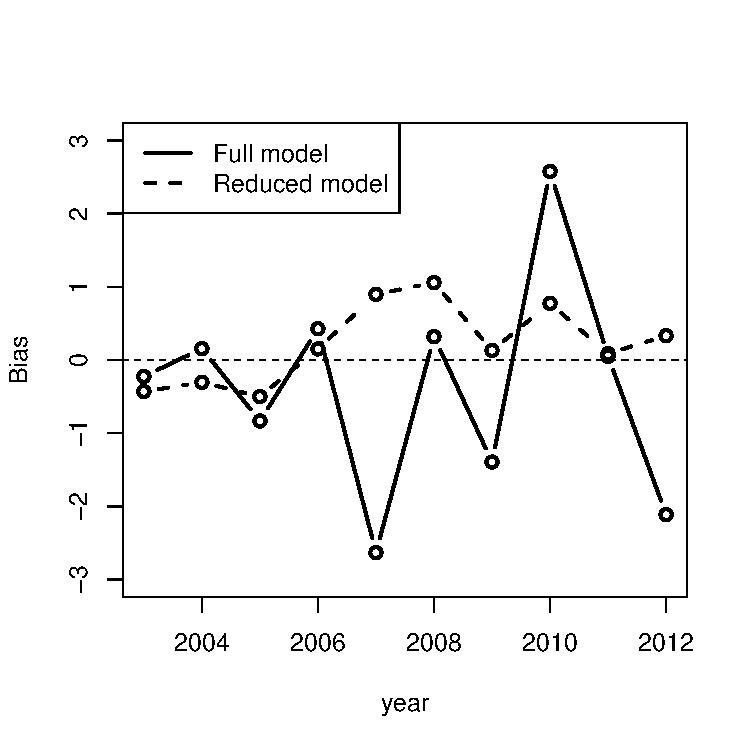
\includegraphics[width=1\linewidth]{rolling_predbias_full_vs_reduced}\\
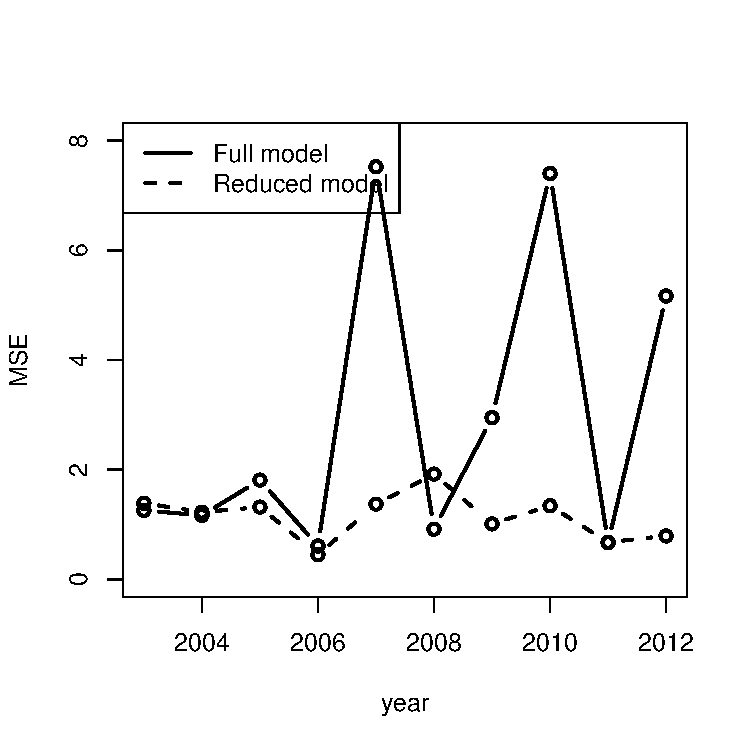
\includegraphics[width=1\linewidth]{rolling_predMSE_full_vs_reduced}\\
\captionof{figure}{Bias and MSE of rolling predictions}
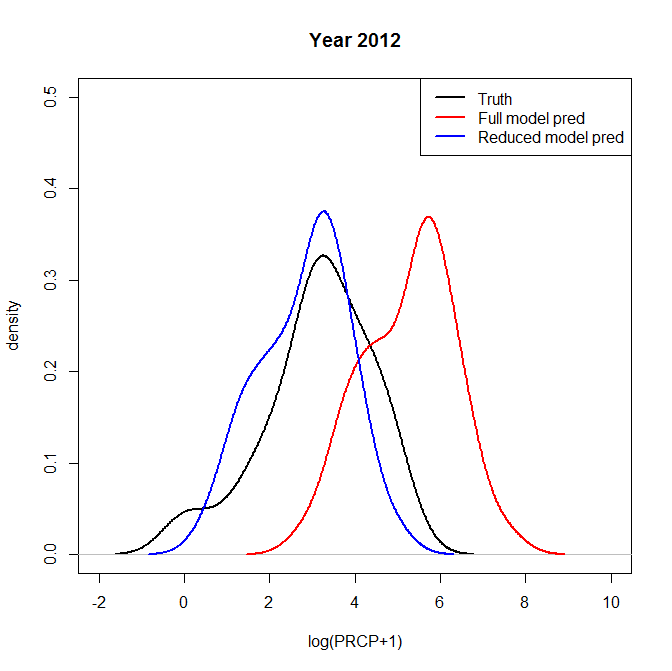
\includegraphics[width=1\linewidth]{rolling_density2012_full_vs_reduced}\\
\vspace{-1em}
\captionof{figure}{Density plots of 2012 predictions and truth}
\end{center}
\end{minipage}
%
\begin{minipage}[b]{.7\textwidth}
\noindent\fbox{
\parbox{\textwidth}{%
{\large {\colbbf Bootstrap scheme}}

\begin{itemize}[leftmargin=*]\compresslist
\vspace{-1em}
\item Wild bootstrap \citep{Mammen93};

\item Say $n$ is total number of observations, $k$ is number of years;

\item Start with estimators from initial LMM: $\hat\bfbeta, \hat\bfgamma, \hat\bfepsilon$;

\item Generate $u^b_\text{WS,year} \stackrel{\text{i.i.d}}{\sim} N(0, n^{0.2}), v^b_\text{year} \stackrel{\text{i.i.d}}{\sim} N(0, k^{0.2})$;

\item Get `new' observations: $ Y^b_\text{WS, year} = \bfx^T_\text{WS, year} \hat\bfbeta + v^b_\text{year} \hat \gamma_\text{year} + u^b_\text{WS, year} \hat\epsilon_\text{WS, year} $
\end{itemize}
\vspace{-1em}
}}

\vspace{2em}
\parbox{.69\textwidth}{
\vspace{-1em}
\begin{center}
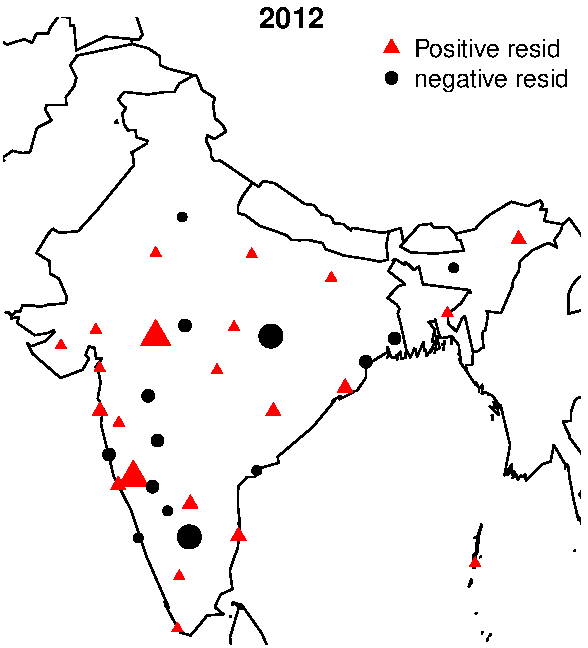
\includegraphics[width=1\linewidth]{rolling_map2012_full_vs_reduced_cropped}
%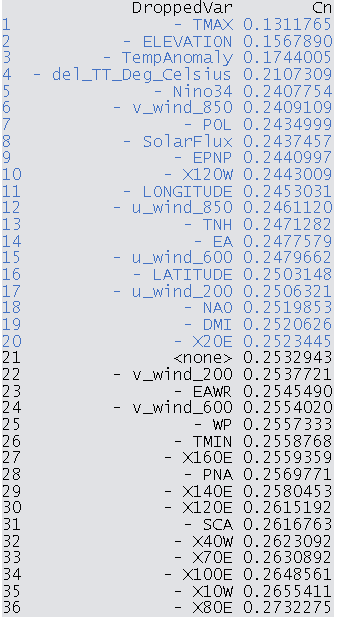
\includegraphics[width=.3\textwidth]{output_cropped}
\captionof{figure}{Stationwise residuals for 2012}
\end{center}
}
%
\parbox{.3\textwidth}{
\vspace{-1em}
\fontsize{6}{7.2}
\selectfont
\begin{tabular}{ll}
\hline
    \textbf{Dropped var}    & \textbf{$C_n$}        \\\hline
    \colorrows{\color{blue}}
    Max temp              & 0.1311765 \\
    Elevation             & 0.156789  \\
    Temp Anomaly          & 0.1744005 \\
    $\Delta TT$ & 0.2107309 \\
    Ni\~{n}o34                & 0.2407754 \\
    $v$-wind 850 mb          & 0.2409109 \\
    POL                   & 0.2434999 \\
    Solar Flux             & 0.2437457 \\
    EPNP                  & 0.2440997 \\
    MJO 120W              & 0.2443009 \\
    Longitude              & 0.2453031 \\
    $u$-wind 850 mb          & 0.246112  \\
    TNH                   & 0.2471282 \\
    EA                    & 0.2477579 \\
    $u$-wind 600 mb          & 0.2479662 \\
    Latitude             & 0.2503148 \\
    $u$-wind 200 mb          & 0.2506321 \\
    NAO                   & 0.2519853 \\
    DMI                   & 0.2520626 \\
    MJO 20E               & 0.2523445 \\\hline
    \colorrows{\color{black}}
    <None>                & 0.2532943 \\\hline
    $v$-wind 200 mb          & 0.2537721 \\
    EAWR                  & 0.254549  \\
    $v$-wind 600 mb          & 0.255402  \\
    WP                    & 0.2557333 \\
    Min temp                  & 0.2558768 \\
    MJO 160E              & 0.2559359 \\
    PNA                   & 0.2569771 \\
    MJO 140E              & 0.2580453 \\
    MJO 120E              & 0.2615192 \\
    SCA                   & 0.2616763 \\
    MJO 40W               & 0.2623092 \\
    MJO 70E               & 0.2630892 \\
    MJO 100E              & 0.2648561 \\
    MJO 10W               & 0.2655411 \\
    MJO 80E               & 0.2732275 \\\hline
\end{tabular}
\captionof{table}{Ordered values of $C_n$ from bootstrap}
}
\vspace{.01em}
\end{minipage}
}

%----------------------------------------------------------------------------------------
%	Discussion
%----------------------------------------------------------------------------------------

\headerbox{Discussion}{name=discussion,column=2,span=2,row=0,below=results}{

\begin{multicols}{2}
\begin{itemize}[leftmargin=*]\compresslist
\item All selected variables (marked in blue in Table 1) have documented effects on Indian monsoon;
 
\item EPNP teleconnection and 120W MJO are both selected: both deal with same longitudinal region;

\item Interesting variables: Solar Flux and Polar/Eurasia teleconnection (POL): an indicator of Eurasian snow cover;

\item TA has a large influence. Several MJO indices, particularly 80E and 40W, are selected when starting from a full model with everything but TA, but are dropped in favor of TA when it is included in the full model;

\item Reduced model predictions have consistently less bias and are more stable across testing years (Figs. 2 and 3). Also there are no spatial patterns in residuals (Fig. 4).
\end{itemize}
\end{multicols}
}

\headerbox{}{name=info,column=2,span=2,row=0,below=discussion,
textborder=none,headerborder=none,boxheaderheight=0pt}{
{\scriptsize
\vspace{-.75em}
\begin{multicols}{2}
\textbf{GitHub}: {\tt https://github.com/shubhobm/Climate-indian-monsoon}

\textbf{Acknowledgement}: NSF grant IIS-1029711;

\textbf{References}:
\vspace{-.7em}
\renewcommand{\section}[2]{\vskip 0.05em} % Get rid of the default "References" section title
\setlength{\bibsep}{0pt plus 0.1ex}
\bibliographystyle{plainnat}
\bibliography{climate}
\end{multicols}
}}

%----------------------------------------------------------------------------------------
%	DATA AND MODELLING
%----------------------------------------------------------------------------------------

\headerbox{Data and modelling}{name=data,column=0,below=objectives,bottomaligned=info}{
% This block's bottom aligns with the bottom of the conclusion block

Annual median observations for 1978-2012;

\vspace{.5em}
\textit{\textbf{Fixed covariates ($\bfx_{p \times 1}, p=35$)}}

\textbf{(A) Station-specific}: (from 36 weather stations across India) Latitude, longitude, elevation, maximum and minimum temperature, tropospheric temperature difference ($\Delta TT$), Indian Dipole Mode Index (DMI), Ni\~{n}o 3.4 anomaly;

\vspace{.25em}
\textbf{(B) Global}:
\vspace{-1em}
\begin{itemize}[leftmargin=*]\compresslist
\item $u$-wind and $v$ wind at 200, 600 and 850 mb;
\item 10 indices of Madden-Julian Oscillations: 20E, 70E, 80E, 100E, 120E, 140E, 160E, 120W, 40W, 10W;
\item Teleconnections: North Atlantic Oscillation (NAO), East Atlantic (EA), West Pacific (WP), East Pacific-North Pacific (EPNP), Pacific/North American (PNA), East Atlantic/Western Russia (EAWR), Scandinavia (SCA), Tropical/Northern Hemisphere (TNH), Polar/Eurasia (POL);
\item Solar Flux;
\item Land-Ocean Temperature Anomaly (TA).
\end{itemize}
%
\textit{\textbf{Random effects ($\bfGamma$)}}: Random intercept by year;

\vspace{.5em}
\textit{\textbf{Linear Mixed Model (LMM):}}

$Y$: log of annual median rainfall at a weather station (WS);

\vspace{-2em}
\begin{eqnarray*}
\text{Level 1:} & & Y_{\text{WS,year}} | \bfGamma=\bfgamma \stackrel{\text{ind}}{\sim} N(\theta_{\text{WS,year}}, \sigma^2);\\
& &\theta_{\text{WS,year}} = \bfx^T_{\text{WS,year}} \bfbeta + \gamma_{\text{year}};\\
\text{Level 2:} & & \Gamma_{\text{year}} \stackrel{\text{i.i.d}}{\sim} N( 0, \tau^2)
\end{eqnarray*}
}

%----------------------------------------------------------------------------------------
%	ALGORITHM
%----------------------------------------------------------------------------------------

\headerbox{The one-step algorithm}{name=algo,bottomaligned=info, column=1,below=methods, boxColorOne=orange!20}{
% This block's bottom aligns with the bottom of the conclusion block

{\colbbf
\begin{enumerate}[leftmargin=*]\compresslist
\item For large enough $n$, Calculate $C_n$ for full model;
\item Drop a predictor, calculate $C_n$ for the reduced model;
\item Repeat for all $p$ predictors;
\item Collect predictors dropping which causes $C_n$ to decrease. These are the predictors in the smallest correct model.
\end{enumerate}
}
}

\end{poster}

\end{document}